% Created by tikzDevice version 0.12.3 on 2020-12-24 12:37:50
% !TEX encoding = UTF-8 Unicode
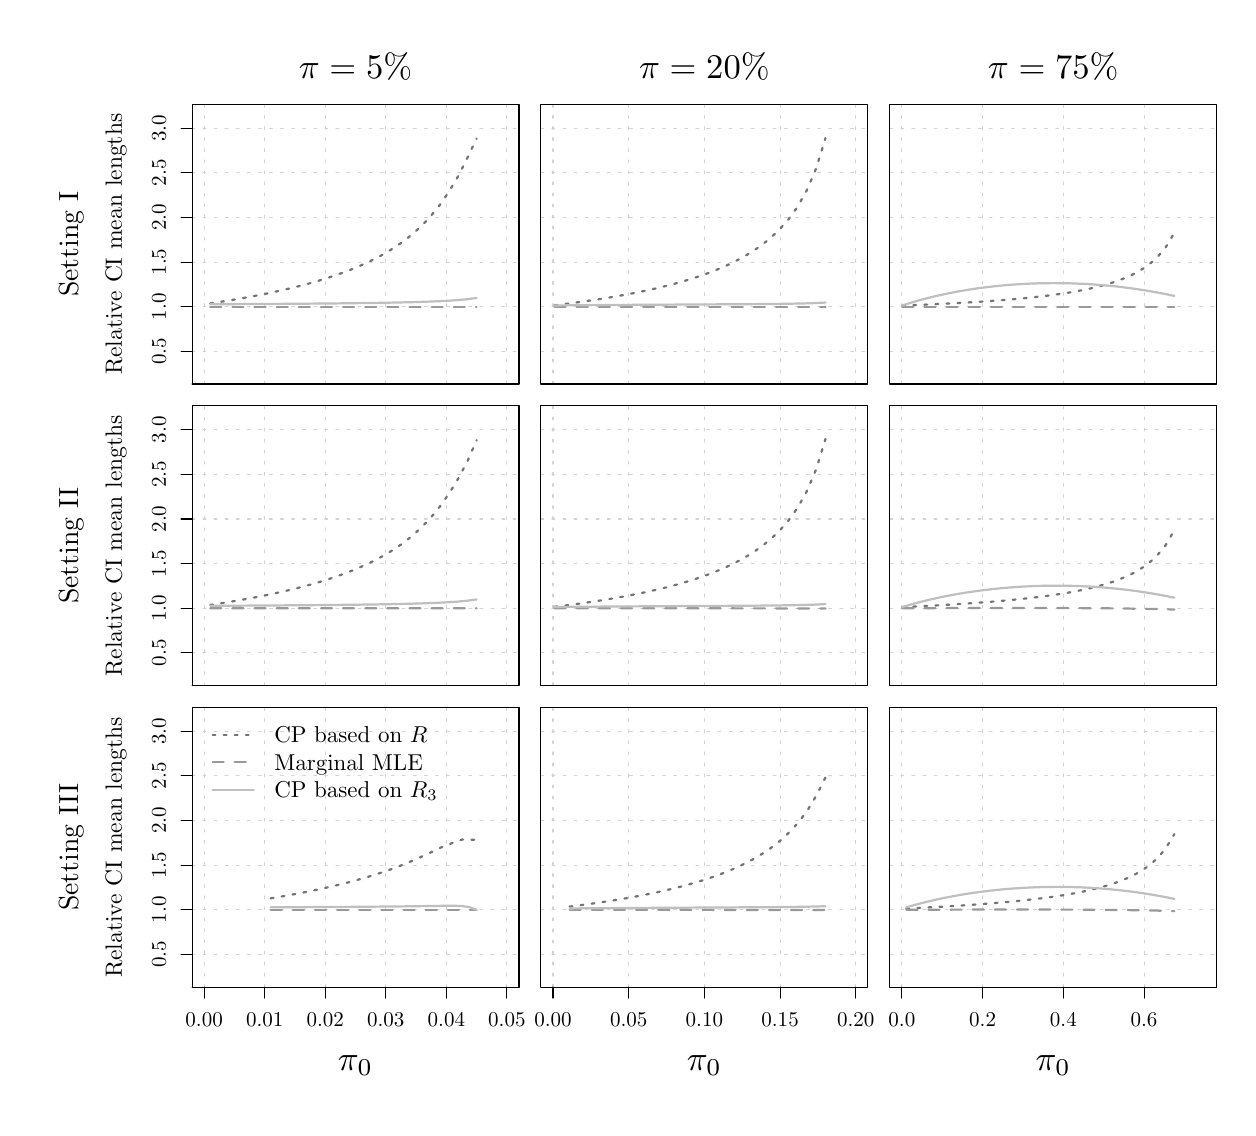
\begin{tikzpicture}[x=1pt,y=1pt]
\definecolor{fillColor}{RGB}{255,255,255}
\path[use as bounding box,fill=fillColor,fill opacity=0.00] (0,0) rectangle (433.62,390.26);
\begin{scope}
\path[clip] ( 55.44,257.53) rectangle (181.50,366.50);
\definecolor{drawColor}{RGB}{0,0,0}

\node[text=drawColor,anchor=base,inner sep=0pt, outer sep=0pt, scale=  0.66] at (118.47,231.40) {Simulation ID};

\node[text=drawColor,rotate= 90.00,anchor=base,inner sep=0pt, outer sep=0pt, scale=  0.66] at ( 34.06,312.01) {Ratio of RMSE};
\end{scope}
\begin{scope}
\path[clip] (  0.00,  0.00) rectangle (433.62,390.26);
\definecolor{drawColor}{RGB}{0,0,0}

\path[draw=drawColor,line width= 0.4pt,line join=round,line cap=round] ( 59.40,273.30) -- ( 59.40,353.96);

\path[draw=drawColor,line width= 0.4pt,line join=round,line cap=round] ( 59.40,273.30) -- ( 55.44,273.30);

\path[draw=drawColor,line width= 0.4pt,line join=round,line cap=round] ( 59.40,289.43) -- ( 55.44,289.43);

\path[draw=drawColor,line width= 0.4pt,line join=round,line cap=round] ( 59.40,305.56) -- ( 55.44,305.56);

\path[draw=drawColor,line width= 0.4pt,line join=round,line cap=round] ( 59.40,321.69) -- ( 55.44,321.69);

\path[draw=drawColor,line width= 0.4pt,line join=round,line cap=round] ( 59.40,337.82) -- ( 55.44,337.82);

\path[draw=drawColor,line width= 0.4pt,line join=round,line cap=round] ( 59.40,353.96) -- ( 55.44,353.96);

\node[text=drawColor,rotate= 90.00,anchor=base,inner sep=0pt, outer sep=0pt, scale=  0.76] at ( 49.90,273.30) {0.5};

\node[text=drawColor,rotate= 90.00,anchor=base,inner sep=0pt, outer sep=0pt, scale=  0.76] at ( 49.90,289.43) {1.0};

\node[text=drawColor,rotate= 90.00,anchor=base,inner sep=0pt, outer sep=0pt, scale=  0.76] at ( 49.90,305.56) {1.5};

\node[text=drawColor,rotate= 90.00,anchor=base,inner sep=0pt, outer sep=0pt, scale=  0.76] at ( 49.90,321.69) {2.0};

\node[text=drawColor,rotate= 90.00,anchor=base,inner sep=0pt, outer sep=0pt, scale=  0.76] at ( 49.90,337.82) {2.5};

\node[text=drawColor,rotate= 90.00,anchor=base,inner sep=0pt, outer sep=0pt, scale=  0.76] at ( 49.90,353.96) {3.0};
\end{scope}
\begin{scope}
\path[clip] ( 59.40,261.49) rectangle (177.54,362.54);
\definecolor{drawColor}{RGB}{211,211,211}

\path[draw=drawColor,line width= 0.4pt,dash pattern=on 1pt off 3pt ,line join=round,line cap=round] ( 63.78,261.49) -- ( 63.78,362.54);

\path[draw=drawColor,line width= 0.4pt,dash pattern=on 1pt off 3pt ,line join=round,line cap=round] ( 85.65,261.49) -- ( 85.65,362.54);

\path[draw=drawColor,line width= 0.4pt,dash pattern=on 1pt off 3pt ,line join=round,line cap=round] (107.53,261.49) -- (107.53,362.54);

\path[draw=drawColor,line width= 0.4pt,dash pattern=on 1pt off 3pt ,line join=round,line cap=round] (129.41,261.49) -- (129.41,362.54);

\path[draw=drawColor,line width= 0.4pt,dash pattern=on 1pt off 3pt ,line join=round,line cap=round] (151.29,261.49) -- (151.29,362.54);

\path[draw=drawColor,line width= 0.4pt,dash pattern=on 1pt off 3pt ,line join=round,line cap=round] (173.16,261.49) -- (173.16,362.54);

\path[draw=drawColor,line width= 0.4pt,dash pattern=on 1pt off 3pt ,line join=round,line cap=round] ( 59.40,273.30) -- (177.54,273.30);

\path[draw=drawColor,line width= 0.4pt,dash pattern=on 1pt off 3pt ,line join=round,line cap=round] ( 59.40,289.43) -- (177.54,289.43);

\path[draw=drawColor,line width= 0.4pt,dash pattern=on 1pt off 3pt ,line join=round,line cap=round] ( 59.40,305.56) -- (177.54,305.56);

\path[draw=drawColor,line width= 0.4pt,dash pattern=on 1pt off 3pt ,line join=round,line cap=round] ( 59.40,321.69) -- (177.54,321.69);

\path[draw=drawColor,line width= 0.4pt,dash pattern=on 1pt off 3pt ,line join=round,line cap=round] ( 59.40,337.82) -- (177.54,337.82);

\path[draw=drawColor,line width= 0.4pt,dash pattern=on 1pt off 3pt ,line join=round,line cap=round] ( 59.40,353.96) -- (177.54,353.96);
\end{scope}
\begin{scope}
\path[clip] (  0.00,  0.00) rectangle (433.62,390.26);
\definecolor{drawColor}{RGB}{0,0,0}

\path[draw=drawColor,line width= 0.4pt,line join=round,line cap=round] ( 59.40,261.49) --
	(177.54,261.49) --
	(177.54,362.54) --
	( 59.40,362.54) --
	( 59.40,261.49);
\end{scope}
\begin{scope}
\path[clip] ( 59.40,261.49) rectangle (177.54,362.54);
\definecolor{drawColor}{gray}{0.45}

\path[draw=drawColor,line width= 0.8pt,dash pattern=on 1pt off 3pt ,line join=round,line cap=round] ( 65.96,290.62) --
	( 69.28,291.13) --
	( 72.60,291.66) --
	( 75.92,292.22) --
	( 79.24,292.81) --
	( 82.56,293.43) --
	( 85.88,294.08) --
	( 89.20,294.78) --
	( 92.52,295.52) --
	( 95.84,296.31) --
	( 99.16,297.15) --
	(102.48,298.04) --
	(105.80,299.01) --
	(109.12,300.07) --
	(112.43,301.19) --
	(115.75,302.41) --
	(119.07,303.75) --
	(122.39,305.23) --
	(125.71,306.86) --
	(129.03,308.66) --
	(132.35,310.68) --
	(135.67,312.98) --
	(138.99,315.60) --
	(142.31,318.62) --
	(145.63,322.12) --
	(148.95,326.22) --
	(152.27,331.05) --
	(155.59,336.65) --
	(158.91,343.22) --
	(162.23,350.22);
\definecolor{drawColor}{gray}{0.60}

\path[draw=drawColor,line width= 0.8pt,dash pattern=on 4pt off 4pt ,line join=round,line cap=round] ( 65.96,289.43) --
	( 69.28,289.43) --
	( 72.60,289.43) --
	( 75.92,289.43) --
	( 79.24,289.43) --
	( 82.56,289.43) --
	( 85.88,289.43) --
	( 89.20,289.43) --
	( 92.52,289.43) --
	( 95.84,289.43) --
	( 99.16,289.43) --
	(102.48,289.43) --
	(105.80,289.43) --
	(109.12,289.43) --
	(112.43,289.43) --
	(115.75,289.43) --
	(119.07,289.43) --
	(122.39,289.43) --
	(125.71,289.43) --
	(129.03,289.43) --
	(132.35,289.43) --
	(135.67,289.43) --
	(138.99,289.43) --
	(142.31,289.43) --
	(145.63,289.43) --
	(148.95,289.43) --
	(152.27,289.43) --
	(155.59,289.43) --
	(158.91,289.43) --
	(162.23,289.43);
\definecolor{drawColor}{gray}{0.75}

\path[draw=drawColor,line width= 0.8pt,line join=round,line cap=round] ( 65.96,290.31) --
	( 69.28,290.33) --
	( 72.60,290.34) --
	( 75.92,290.36) --
	( 79.24,290.38) --
	( 82.56,290.40) --
	( 85.88,290.42) --
	( 89.20,290.44) --
	( 92.52,290.46) --
	( 95.84,290.48) --
	( 99.16,290.51) --
	(102.48,290.54) --
	(105.80,290.57) --
	(109.12,290.60) --
	(112.43,290.63) --
	(115.75,290.67) --
	(119.07,290.71) --
	(122.39,290.75) --
	(125.71,290.80) --
	(129.03,290.85) --
	(132.35,290.92) --
	(135.67,290.99) --
	(138.99,291.07) --
	(142.31,291.17) --
	(145.63,291.29) --
	(148.95,291.43) --
	(152.27,291.60) --
	(155.59,291.83) --
	(158.91,292.14) --
	(162.23,292.60);
\end{scope}
\begin{scope}
\path[clip] (  0.00,  0.00) rectangle (433.62,390.26);
\definecolor{drawColor}{RGB}{0,0,0}

\node[text=drawColor,rotate= 90.00,anchor=base,inner sep=0pt, outer sep=0pt, scale=  1.00] at ( 18.22,312.01) {Setting I};

\node[text=drawColor,rotate= 90.00,anchor=base,inner sep=0pt, outer sep=0pt, scale=  0.85] at ( 34.06,312.01) {Relative CI mean lengths};

\node[text=drawColor,anchor=base,inner sep=0pt, outer sep=0pt, scale=  1.25] at (118.47,372.04) {$\pi = 5\%$};
\end{scope}
\begin{scope}
\path[clip] (181.50,257.53) rectangle (307.56,366.50);
\definecolor{drawColor}{RGB}{0,0,0}

\node[text=drawColor,anchor=base,inner sep=0pt, outer sep=0pt, scale=  0.66] at (244.53,231.40) {Simulation ID};

\node[text=drawColor,rotate= 90.00,anchor=base,inner sep=0pt, outer sep=0pt, scale=  0.66] at (160.12,312.01) {Ratio of RMSE};
\end{scope}
\begin{scope}
\path[clip] (185.46,261.49) rectangle (303.60,362.54);
\definecolor{drawColor}{RGB}{211,211,211}

\path[draw=drawColor,line width= 0.4pt,dash pattern=on 1pt off 3pt ,line join=round,line cap=round] (189.84,261.49) -- (189.84,362.54);

\path[draw=drawColor,line width= 0.4pt,dash pattern=on 1pt off 3pt ,line join=round,line cap=round] (217.18,261.49) -- (217.18,362.54);

\path[draw=drawColor,line width= 0.4pt,dash pattern=on 1pt off 3pt ,line join=round,line cap=round] (244.53,261.49) -- (244.53,362.54);

\path[draw=drawColor,line width= 0.4pt,dash pattern=on 1pt off 3pt ,line join=round,line cap=round] (271.88,261.49) -- (271.88,362.54);

\path[draw=drawColor,line width= 0.4pt,dash pattern=on 1pt off 3pt ,line join=round,line cap=round] (299.22,261.49) -- (299.22,362.54);

\path[draw=drawColor,line width= 0.4pt,dash pattern=on 1pt off 3pt ,line join=round,line cap=round] (185.46,273.30) -- (303.60,273.30);

\path[draw=drawColor,line width= 0.4pt,dash pattern=on 1pt off 3pt ,line join=round,line cap=round] (185.46,289.43) -- (303.60,289.43);

\path[draw=drawColor,line width= 0.4pt,dash pattern=on 1pt off 3pt ,line join=round,line cap=round] (185.46,305.56) -- (303.60,305.56);

\path[draw=drawColor,line width= 0.4pt,dash pattern=on 1pt off 3pt ,line join=round,line cap=round] (185.46,321.69) -- (303.60,321.69);

\path[draw=drawColor,line width= 0.4pt,dash pattern=on 1pt off 3pt ,line join=round,line cap=round] (185.46,337.82) -- (303.60,337.82);

\path[draw=drawColor,line width= 0.4pt,dash pattern=on 1pt off 3pt ,line join=round,line cap=round] (185.46,353.96) -- (303.60,353.96);
\end{scope}
\begin{scope}
\path[clip] (  0.00,  0.00) rectangle (433.62,390.26);
\definecolor{drawColor}{RGB}{0,0,0}

\path[draw=drawColor,line width= 0.4pt,line join=round,line cap=round] (185.46,261.49) --
	(303.60,261.49) --
	(303.60,362.54) --
	(185.46,362.54) --
	(185.46,261.49);
\end{scope}
\begin{scope}
\path[clip] (185.46,261.49) rectangle (303.60,362.54);
\definecolor{drawColor}{gray}{0.45}

\path[draw=drawColor,line width= 0.8pt,dash pattern=on 1pt off 3pt ,line join=round,line cap=round] (190.38,289.94) --
	(193.76,290.36) --
	(197.13,290.80) --
	(200.51,291.26) --
	(203.89,291.75) --
	(207.26,292.27) --
	(210.64,292.82) --
	(214.01,293.40) --
	(217.39,294.03) --
	(220.77,294.69) --
	(224.14,295.40) --
	(227.52,296.16) --
	(230.89,296.98) --
	(234.27,297.87) --
	(237.65,298.83) --
	(241.02,299.88) --
	(244.40,301.02) --
	(247.77,302.28) --
	(251.15,303.68) --
	(254.53,305.24) --
	(257.90,306.99) --
	(261.28,308.98) --
	(264.65,311.26) --
	(268.03,313.91) --
	(271.41,317.05) --
	(274.78,320.82) --
	(278.16,325.50) --
	(281.53,331.48) --
	(284.91,339.42) --
	(288.29,350.35);
\definecolor{drawColor}{gray}{0.60}

\path[draw=drawColor,line width= 0.8pt,dash pattern=on 4pt off 4pt ,line join=round,line cap=round] (190.38,289.43) --
	(193.76,289.43) --
	(197.13,289.43) --
	(200.51,289.43) --
	(203.89,289.43) --
	(207.26,289.43) --
	(210.64,289.43) --
	(214.01,289.43) --
	(217.39,289.43) --
	(220.77,289.43) --
	(224.14,289.43) --
	(227.52,289.43) --
	(230.89,289.43) --
	(234.27,289.43) --
	(237.65,289.43) --
	(241.02,289.43) --
	(244.40,289.43) --
	(247.77,289.43) --
	(251.15,289.43) --
	(254.53,289.43) --
	(257.90,289.43) --
	(261.28,289.43) --
	(264.65,289.43) --
	(268.03,289.43) --
	(271.41,289.43) --
	(274.78,289.43) --
	(278.16,289.43) --
	(281.53,289.43) --
	(284.91,289.43) --
	(288.29,289.43);
\definecolor{drawColor}{gray}{0.75}

\path[draw=drawColor,line width= 0.8pt,line join=round,line cap=round] (190.38,289.88) --
	(193.76,289.91) --
	(197.13,289.94) --
	(200.51,289.97) --
	(203.89,290.00) --
	(207.26,290.02) --
	(210.64,290.05) --
	(214.01,290.07) --
	(217.39,290.09) --
	(220.77,290.11) --
	(224.14,290.13) --
	(227.52,290.15) --
	(230.89,290.17) --
	(234.27,290.19) --
	(237.65,290.21) --
	(241.02,290.23) --
	(244.40,290.25) --
	(247.77,290.27) --
	(251.15,290.29) --
	(254.53,290.31) --
	(257.90,290.33) --
	(261.28,290.35) --
	(264.65,290.38) --
	(268.03,290.41) --
	(271.41,290.45) --
	(274.78,290.50) --
	(278.16,290.56) --
	(281.53,290.64) --
	(284.91,290.75) --
	(288.29,290.93);
\end{scope}
\begin{scope}
\path[clip] (  0.00,  0.00) rectangle (433.62,390.26);
\definecolor{drawColor}{RGB}{0,0,0}

\node[text=drawColor,anchor=base,inner sep=0pt, outer sep=0pt, scale=  1.25] at (244.53,372.04) {$\pi = 20\%$};
\end{scope}
\begin{scope}
\path[clip] (307.56,257.53) rectangle (433.62,366.50);
\definecolor{drawColor}{RGB}{0,0,0}

\node[text=drawColor,anchor=base,inner sep=0pt, outer sep=0pt, scale=  0.66] at (370.59,231.40) {Simulation ID};

\node[text=drawColor,rotate= 90.00,anchor=base,inner sep=0pt, outer sep=0pt, scale=  0.66] at (286.18,312.01) {Ratio of RMSE};
\end{scope}
\begin{scope}
\path[clip] (311.52,261.49) rectangle (429.66,362.54);
\definecolor{drawColor}{RGB}{211,211,211}

\path[draw=drawColor,line width= 0.4pt,dash pattern=on 1pt off 3pt ,line join=round,line cap=round] (315.90,261.49) -- (315.90,362.54);

\path[draw=drawColor,line width= 0.4pt,dash pattern=on 1pt off 3pt ,line join=round,line cap=round] (345.07,261.49) -- (345.07,362.54);

\path[draw=drawColor,line width= 0.4pt,dash pattern=on 1pt off 3pt ,line join=round,line cap=round] (374.24,261.49) -- (374.24,362.54);

\path[draw=drawColor,line width= 0.4pt,dash pattern=on 1pt off 3pt ,line join=round,line cap=round] (403.41,261.49) -- (403.41,362.54);

\path[draw=drawColor,line width= 0.4pt,dash pattern=on 1pt off 3pt ,line join=round,line cap=round] (311.52,273.30) -- (429.66,273.30);

\path[draw=drawColor,line width= 0.4pt,dash pattern=on 1pt off 3pt ,line join=round,line cap=round] (311.52,289.43) -- (429.66,289.43);

\path[draw=drawColor,line width= 0.4pt,dash pattern=on 1pt off 3pt ,line join=round,line cap=round] (311.52,305.56) -- (429.66,305.56);

\path[draw=drawColor,line width= 0.4pt,dash pattern=on 1pt off 3pt ,line join=round,line cap=round] (311.52,321.69) -- (429.66,321.69);

\path[draw=drawColor,line width= 0.4pt,dash pattern=on 1pt off 3pt ,line join=round,line cap=round] (311.52,337.82) -- (429.66,337.82);

\path[draw=drawColor,line width= 0.4pt,dash pattern=on 1pt off 3pt ,line join=round,line cap=round] (311.52,353.96) -- (429.66,353.96);
\end{scope}
\begin{scope}
\path[clip] (  0.00,  0.00) rectangle (433.62,390.26);
\definecolor{drawColor}{RGB}{0,0,0}

\path[draw=drawColor,line width= 0.4pt,line join=round,line cap=round] (311.52,261.49) --
	(429.66,261.49) --
	(429.66,362.54) --
	(311.52,362.54) --
	(311.52,261.49);
\end{scope}
\begin{scope}
\path[clip] (311.52,261.49) rectangle (429.66,362.54);
\definecolor{drawColor}{gray}{0.45}

\path[draw=drawColor,line width= 0.8pt,dash pattern=on 1pt off 3pt ,line join=round,line cap=round] (316.04,289.84) --
	(319.43,289.98) --
	(322.82,290.11) --
	(326.21,290.26) --
	(329.60,290.42) --
	(332.99,290.59) --
	(336.38,290.77) --
	(339.77,290.96) --
	(343.16,291.17) --
	(346.55,291.39) --
	(349.94,291.64) --
	(353.33,291.90) --
	(356.72,292.19) --
	(360.11,292.51) --
	(363.50,292.85) --
	(366.89,293.23) --
	(370.28,293.66) --
	(373.67,294.13) --
	(377.06,294.67) --
	(380.45,295.28) --
	(383.84,295.97) --
	(387.23,296.77) --
	(390.62,297.70) --
	(394.01,298.81) --
	(397.40,300.16) --
	(400.79,301.81) --
	(404.18,303.91) --
	(407.57,306.66) --
	(410.96,310.47) --
	(414.35,316.11);
\definecolor{drawColor}{gray}{0.60}

\path[draw=drawColor,line width= 0.8pt,dash pattern=on 4pt off 4pt ,line join=round,line cap=round] (316.04,289.43) --
	(319.43,289.43) --
	(322.82,289.43) --
	(326.21,289.43) --
	(329.60,289.43) --
	(332.99,289.43) --
	(336.38,289.43) --
	(339.77,289.43) --
	(343.16,289.43) --
	(346.55,289.43) --
	(349.94,289.43) --
	(353.33,289.43) --
	(356.72,289.43) --
	(360.11,289.43) --
	(363.50,289.43) --
	(366.89,289.43) --
	(370.28,289.43) --
	(373.67,289.43) --
	(377.06,289.43) --
	(380.45,289.43) --
	(383.84,289.43) --
	(387.23,289.43) --
	(390.62,289.43) --
	(394.01,289.43) --
	(397.40,289.43) --
	(400.79,289.43) --
	(404.18,289.43) --
	(407.57,289.43) --
	(410.96,289.43) --
	(414.35,289.43);
\definecolor{drawColor}{gray}{0.75}

\path[draw=drawColor,line width= 0.8pt,line join=round,line cap=round] (316.04,289.89) --
	(319.43,290.96) --
	(322.82,291.93) --
	(326.21,292.81) --
	(329.60,293.60) --
	(332.99,294.32) --
	(336.38,294.97) --
	(339.77,295.54) --
	(343.16,296.05) --
	(346.55,296.49) --
	(349.94,296.88) --
	(353.33,297.20) --
	(356.72,297.46) --
	(360.11,297.67) --
	(363.50,297.82) --
	(366.89,297.91) --
	(370.28,297.95) --
	(373.67,297.93) --
	(377.06,297.86) --
	(380.45,297.74) --
	(383.84,297.56) --
	(387.23,297.32) --
	(390.62,297.03) --
	(394.01,296.68) --
	(397.40,296.26) --
	(400.79,295.79) --
	(404.18,295.26) --
	(407.57,294.67) --
	(410.96,294.03) --
	(414.35,293.33);
\end{scope}
\begin{scope}
\path[clip] (  0.00,  0.00) rectangle (433.62,390.26);
\definecolor{drawColor}{RGB}{0,0,0}

\node[text=drawColor,anchor=base,inner sep=0pt, outer sep=0pt, scale=  1.25] at (370.59,372.04) {$\pi = 75\%$};
\end{scope}
\begin{scope}
\path[clip] ( 55.44,148.57) rectangle (181.50,257.53);
\definecolor{drawColor}{RGB}{0,0,0}

\node[text=drawColor,anchor=base,inner sep=0pt, outer sep=0pt, scale=  0.66] at (118.47,122.43) {Simulation ID};

\node[text=drawColor,rotate= 90.00,anchor=base,inner sep=0pt, outer sep=0pt, scale=  0.66] at ( 34.06,203.05) {Ratio of RMSE};
\end{scope}
\begin{scope}
\path[clip] (  0.00,  0.00) rectangle (433.62,390.26);
\definecolor{drawColor}{RGB}{0,0,0}

\path[draw=drawColor,line width= 0.4pt,line join=round,line cap=round] ( 59.40,164.33) -- ( 59.40,244.99);

\path[draw=drawColor,line width= 0.4pt,line join=round,line cap=round] ( 59.40,164.33) -- ( 55.44,164.33);

\path[draw=drawColor,line width= 0.4pt,line join=round,line cap=round] ( 59.40,180.47) -- ( 55.44,180.47);

\path[draw=drawColor,line width= 0.4pt,line join=round,line cap=round] ( 59.40,196.60) -- ( 55.44,196.60);

\path[draw=drawColor,line width= 0.4pt,line join=round,line cap=round] ( 59.40,212.73) -- ( 55.44,212.73);

\path[draw=drawColor,line width= 0.4pt,line join=round,line cap=round] ( 59.40,228.86) -- ( 55.44,228.86);

\path[draw=drawColor,line width= 0.4pt,line join=round,line cap=round] ( 59.40,244.99) -- ( 55.44,244.99);

\node[text=drawColor,rotate= 90.00,anchor=base,inner sep=0pt, outer sep=0pt, scale=  0.76] at ( 49.90,164.33) {0.5};

\node[text=drawColor,rotate= 90.00,anchor=base,inner sep=0pt, outer sep=0pt, scale=  0.76] at ( 49.90,180.47) {1.0};

\node[text=drawColor,rotate= 90.00,anchor=base,inner sep=0pt, outer sep=0pt, scale=  0.76] at ( 49.90,196.60) {1.5};

\node[text=drawColor,rotate= 90.00,anchor=base,inner sep=0pt, outer sep=0pt, scale=  0.76] at ( 49.90,212.73) {2.0};

\node[text=drawColor,rotate= 90.00,anchor=base,inner sep=0pt, outer sep=0pt, scale=  0.76] at ( 49.90,228.86) {2.5};

\node[text=drawColor,rotate= 90.00,anchor=base,inner sep=0pt, outer sep=0pt, scale=  0.76] at ( 49.90,244.99) {3.0};
\end{scope}
\begin{scope}
\path[clip] ( 59.40,152.53) rectangle (177.54,253.57);
\definecolor{drawColor}{RGB}{211,211,211}

\path[draw=drawColor,line width= 0.4pt,dash pattern=on 1pt off 3pt ,line join=round,line cap=round] ( 63.78,152.53) -- ( 63.78,253.57);

\path[draw=drawColor,line width= 0.4pt,dash pattern=on 1pt off 3pt ,line join=round,line cap=round] ( 85.65,152.53) -- ( 85.65,253.57);

\path[draw=drawColor,line width= 0.4pt,dash pattern=on 1pt off 3pt ,line join=round,line cap=round] (107.53,152.53) -- (107.53,253.57);

\path[draw=drawColor,line width= 0.4pt,dash pattern=on 1pt off 3pt ,line join=round,line cap=round] (129.41,152.53) -- (129.41,253.57);

\path[draw=drawColor,line width= 0.4pt,dash pattern=on 1pt off 3pt ,line join=round,line cap=round] (151.29,152.53) -- (151.29,253.57);

\path[draw=drawColor,line width= 0.4pt,dash pattern=on 1pt off 3pt ,line join=round,line cap=round] (173.16,152.53) -- (173.16,253.57);

\path[draw=drawColor,line width= 0.4pt,dash pattern=on 1pt off 3pt ,line join=round,line cap=round] ( 59.40,164.33) -- (177.54,164.33);

\path[draw=drawColor,line width= 0.4pt,dash pattern=on 1pt off 3pt ,line join=round,line cap=round] ( 59.40,180.47) -- (177.54,180.47);

\path[draw=drawColor,line width= 0.4pt,dash pattern=on 1pt off 3pt ,line join=round,line cap=round] ( 59.40,196.60) -- (177.54,196.60);

\path[draw=drawColor,line width= 0.4pt,dash pattern=on 1pt off 3pt ,line join=round,line cap=round] ( 59.40,212.73) -- (177.54,212.73);

\path[draw=drawColor,line width= 0.4pt,dash pattern=on 1pt off 3pt ,line join=round,line cap=round] ( 59.40,228.86) -- (177.54,228.86);

\path[draw=drawColor,line width= 0.4pt,dash pattern=on 1pt off 3pt ,line join=round,line cap=round] ( 59.40,244.99) -- (177.54,244.99);
\end{scope}
\begin{scope}
\path[clip] (  0.00,  0.00) rectangle (433.62,390.26);
\definecolor{drawColor}{RGB}{0,0,0}

\path[draw=drawColor,line width= 0.4pt,line join=round,line cap=round] ( 59.40,152.53) --
	(177.54,152.53) --
	(177.54,253.57) --
	( 59.40,253.57) --
	( 59.40,152.53);
\end{scope}
\begin{scope}
\path[clip] ( 59.40,152.53) rectangle (177.54,253.57);
\definecolor{drawColor}{gray}{0.45}

\path[draw=drawColor,line width= 0.8pt,dash pattern=on 1pt off 3pt ,line join=round,line cap=round] ( 65.96,181.66) --
	( 69.28,182.17) --
	( 72.60,182.70) --
	( 75.92,183.26) --
	( 79.24,183.85) --
	( 82.56,184.47) --
	( 85.88,185.13) --
	( 89.20,185.83) --
	( 92.52,186.57) --
	( 95.84,187.36) --
	( 99.16,188.19) --
	(102.48,189.09) --
	(105.80,190.06) --
	(109.12,191.12) --
	(112.43,192.25) --
	(115.75,193.46) --
	(119.07,194.81) --
	(122.39,196.30) --
	(125.71,197.91) --
	(129.03,199.72) --
	(132.35,201.74) --
	(135.67,204.03) --
	(138.99,206.66) --
	(142.31,209.67) --
	(145.63,213.15) --
	(148.95,217.21) --
	(152.27,221.91) --
	(155.59,227.35) --
	(158.91,233.60) --
	(162.23,241.20);
\definecolor{drawColor}{gray}{0.60}

\path[draw=drawColor,line width= 0.8pt,dash pattern=on 4pt off 4pt ,line join=round,line cap=round] ( 65.96,180.46) --
	( 69.28,180.46) --
	( 72.60,180.46) --
	( 75.92,180.46) --
	( 79.24,180.46) --
	( 82.56,180.46) --
	( 85.88,180.46) --
	( 89.20,180.46) --
	( 92.52,180.46) --
	( 95.84,180.46) --
	( 99.16,180.46) --
	(102.48,180.46) --
	(105.80,180.46) --
	(109.12,180.46) --
	(112.43,180.46) --
	(115.75,180.46) --
	(119.07,180.46) --
	(122.39,180.46) --
	(125.71,180.46) --
	(129.03,180.46) --
	(132.35,180.45) --
	(135.67,180.45) --
	(138.99,180.45) --
	(142.31,180.45) --
	(145.63,180.45) --
	(148.95,180.45) --
	(152.27,180.45) --
	(155.59,180.45) --
	(158.91,180.45) --
	(162.23,180.45);
\definecolor{drawColor}{gray}{0.75}

\path[draw=drawColor,line width= 0.8pt,line join=round,line cap=round] ( 65.96,181.35) --
	( 69.28,181.37) --
	( 72.60,181.39) --
	( 75.92,181.40) --
	( 79.24,181.42) --
	( 82.56,181.44) --
	( 85.88,181.46) --
	( 89.20,181.48) --
	( 92.52,181.51) --
	( 95.84,181.53) --
	( 99.16,181.56) --
	(102.48,181.58) --
	(105.80,181.61) --
	(109.12,181.64) --
	(112.43,181.68) --
	(115.75,181.71) --
	(119.07,181.75) --
	(122.39,181.80) --
	(125.71,181.85) --
	(129.03,181.90) --
	(132.35,181.97) --
	(135.67,182.04) --
	(138.99,182.12) --
	(142.31,182.22) --
	(145.63,182.33) --
	(148.95,182.48) --
	(152.27,182.66) --
	(155.59,182.89) --
	(158.91,183.20) --
	(162.23,183.65);
\end{scope}
\begin{scope}
\path[clip] (  0.00,  0.00) rectangle (433.62,390.26);
\definecolor{drawColor}{RGB}{0,0,0}

\node[text=drawColor,rotate= 90.00,anchor=base,inner sep=0pt, outer sep=0pt, scale=  1.00] at ( 18.22,203.05) {Setting II};

\node[text=drawColor,rotate= 90.00,anchor=base,inner sep=0pt, outer sep=0pt, scale=  0.85] at ( 34.06,203.05) {Relative CI mean lengths};
\end{scope}
\begin{scope}
\path[clip] (181.50,148.57) rectangle (307.56,257.53);
\definecolor{drawColor}{RGB}{0,0,0}

\node[text=drawColor,anchor=base,inner sep=0pt, outer sep=0pt, scale=  0.66] at (244.53,122.43) {Simulation ID};

\node[text=drawColor,rotate= 90.00,anchor=base,inner sep=0pt, outer sep=0pt, scale=  0.66] at (160.12,203.05) {Ratio of RMSE};
\end{scope}
\begin{scope}
\path[clip] (185.46,152.53) rectangle (303.60,253.57);
\definecolor{drawColor}{RGB}{211,211,211}

\path[draw=drawColor,line width= 0.4pt,dash pattern=on 1pt off 3pt ,line join=round,line cap=round] (189.84,152.53) -- (189.84,253.57);

\path[draw=drawColor,line width= 0.4pt,dash pattern=on 1pt off 3pt ,line join=round,line cap=round] (217.18,152.53) -- (217.18,253.57);

\path[draw=drawColor,line width= 0.4pt,dash pattern=on 1pt off 3pt ,line join=round,line cap=round] (244.53,152.53) -- (244.53,253.57);

\path[draw=drawColor,line width= 0.4pt,dash pattern=on 1pt off 3pt ,line join=round,line cap=round] (271.88,152.53) -- (271.88,253.57);

\path[draw=drawColor,line width= 0.4pt,dash pattern=on 1pt off 3pt ,line join=round,line cap=round] (299.22,152.53) -- (299.22,253.57);

\path[draw=drawColor,line width= 0.4pt,dash pattern=on 1pt off 3pt ,line join=round,line cap=round] (185.46,164.33) -- (303.60,164.33);

\path[draw=drawColor,line width= 0.4pt,dash pattern=on 1pt off 3pt ,line join=round,line cap=round] (185.46,180.47) -- (303.60,180.47);

\path[draw=drawColor,line width= 0.4pt,dash pattern=on 1pt off 3pt ,line join=round,line cap=round] (185.46,196.60) -- (303.60,196.60);

\path[draw=drawColor,line width= 0.4pt,dash pattern=on 1pt off 3pt ,line join=round,line cap=round] (185.46,212.73) -- (303.60,212.73);

\path[draw=drawColor,line width= 0.4pt,dash pattern=on 1pt off 3pt ,line join=round,line cap=round] (185.46,228.86) -- (303.60,228.86);

\path[draw=drawColor,line width= 0.4pt,dash pattern=on 1pt off 3pt ,line join=round,line cap=round] (185.46,244.99) -- (303.60,244.99);
\end{scope}
\begin{scope}
\path[clip] (  0.00,  0.00) rectangle (433.62,390.26);
\definecolor{drawColor}{RGB}{0,0,0}

\path[draw=drawColor,line width= 0.4pt,line join=round,line cap=round] (185.46,152.53) --
	(303.60,152.53) --
	(303.60,253.57) --
	(185.46,253.57) --
	(185.46,152.53);
\end{scope}
\begin{scope}
\path[clip] (185.46,152.53) rectangle (303.60,253.57);
\definecolor{drawColor}{gray}{0.45}

\path[draw=drawColor,line width= 0.8pt,dash pattern=on 1pt off 3pt ,line join=round,line cap=round] (190.38,180.98) --
	(193.76,181.40) --
	(197.13,181.84) --
	(200.51,182.31) --
	(203.89,182.80) --
	(207.26,183.32) --
	(210.64,183.88) --
	(214.01,184.46) --
	(217.39,185.09) --
	(220.77,185.75) --
	(224.14,186.47) --
	(227.52,187.23) --
	(230.89,188.05) --
	(234.27,188.94) --
	(237.65,189.91) --
	(241.02,190.96) --
	(244.40,192.11) --
	(247.77,193.38) --
	(251.15,194.78) --
	(254.53,196.34) --
	(257.90,198.10) --
	(261.28,200.10) --
	(264.65,202.39) --
	(268.03,205.06) --
	(271.41,208.20) --
	(274.78,211.99) --
	(278.16,216.69) --
	(281.53,222.70) --
	(284.91,230.66) --
	(288.29,241.64);
\definecolor{drawColor}{gray}{0.60}

\path[draw=drawColor,line width= 0.8pt,dash pattern=on 4pt off 4pt ,line join=round,line cap=round] (190.38,180.47) --
	(193.76,180.46) --
	(197.13,180.46) --
	(200.51,180.46) --
	(203.89,180.46) --
	(207.26,180.46) --
	(210.64,180.46) --
	(214.01,180.45) --
	(217.39,180.45) --
	(220.77,180.45) --
	(224.14,180.45) --
	(227.52,180.45) --
	(230.89,180.44) --
	(234.27,180.44) --
	(237.65,180.44) --
	(241.02,180.44) --
	(244.40,180.43) --
	(247.77,180.43) --
	(251.15,180.43) --
	(254.53,180.43) --
	(257.90,180.42) --
	(261.28,180.42) --
	(264.65,180.42) --
	(268.03,180.42) --
	(271.41,180.41) --
	(274.78,180.41) --
	(278.16,180.41) --
	(281.53,180.40) --
	(284.91,180.40) --
	(288.29,180.40);
\definecolor{drawColor}{gray}{0.75}

\path[draw=drawColor,line width= 0.8pt,line join=round,line cap=round] (190.38,180.92) --
	(193.76,180.95) --
	(197.13,180.98) --
	(200.51,181.01) --
	(203.89,181.03) --
	(207.26,181.06) --
	(210.64,181.08) --
	(214.01,181.10) --
	(217.39,181.13) --
	(220.77,181.15) --
	(224.14,181.17) --
	(227.52,181.19) --
	(230.89,181.21) --
	(234.27,181.23) --
	(237.65,181.25) --
	(241.02,181.26) --
	(244.40,181.28) --
	(247.77,181.30) --
	(251.15,181.32) --
	(254.53,181.34) --
	(257.90,181.37) --
	(261.28,181.39) --
	(264.65,181.42) --
	(268.03,181.45) --
	(271.41,181.49) --
	(274.78,181.54) --
	(278.16,181.60) --
	(281.53,181.68) --
	(284.91,181.80) --
	(288.29,181.98);
\end{scope}
\begin{scope}
\path[clip] (307.56,148.57) rectangle (433.62,257.53);
\definecolor{drawColor}{RGB}{0,0,0}

\node[text=drawColor,anchor=base,inner sep=0pt, outer sep=0pt, scale=  0.66] at (370.59,122.43) {Simulation ID};

\node[text=drawColor,rotate= 90.00,anchor=base,inner sep=0pt, outer sep=0pt, scale=  0.66] at (286.18,203.05) {Ratio of RMSE};
\end{scope}
\begin{scope}
\path[clip] (311.52,152.53) rectangle (429.66,253.57);
\definecolor{drawColor}{RGB}{211,211,211}

\path[draw=drawColor,line width= 0.4pt,dash pattern=on 1pt off 3pt ,line join=round,line cap=round] (315.90,152.53) -- (315.90,253.57);

\path[draw=drawColor,line width= 0.4pt,dash pattern=on 1pt off 3pt ,line join=round,line cap=round] (345.07,152.53) -- (345.07,253.57);

\path[draw=drawColor,line width= 0.4pt,dash pattern=on 1pt off 3pt ,line join=round,line cap=round] (374.24,152.53) -- (374.24,253.57);

\path[draw=drawColor,line width= 0.4pt,dash pattern=on 1pt off 3pt ,line join=round,line cap=round] (403.41,152.53) -- (403.41,253.57);

\path[draw=drawColor,line width= 0.4pt,dash pattern=on 1pt off 3pt ,line join=round,line cap=round] (311.52,164.33) -- (429.66,164.33);

\path[draw=drawColor,line width= 0.4pt,dash pattern=on 1pt off 3pt ,line join=round,line cap=round] (311.52,180.47) -- (429.66,180.47);

\path[draw=drawColor,line width= 0.4pt,dash pattern=on 1pt off 3pt ,line join=round,line cap=round] (311.52,196.60) -- (429.66,196.60);

\path[draw=drawColor,line width= 0.4pt,dash pattern=on 1pt off 3pt ,line join=round,line cap=round] (311.52,212.73) -- (429.66,212.73);

\path[draw=drawColor,line width= 0.4pt,dash pattern=on 1pt off 3pt ,line join=round,line cap=round] (311.52,228.86) -- (429.66,228.86);

\path[draw=drawColor,line width= 0.4pt,dash pattern=on 1pt off 3pt ,line join=round,line cap=round] (311.52,244.99) -- (429.66,244.99);
\end{scope}
\begin{scope}
\path[clip] (  0.00,  0.00) rectangle (433.62,390.26);
\definecolor{drawColor}{RGB}{0,0,0}

\path[draw=drawColor,line width= 0.4pt,line join=round,line cap=round] (311.52,152.53) --
	(429.66,152.53) --
	(429.66,253.57) --
	(311.52,253.57) --
	(311.52,152.53);
\end{scope}
\begin{scope}
\path[clip] (311.52,152.53) rectangle (429.66,253.57);
\definecolor{drawColor}{gray}{0.45}

\path[draw=drawColor,line width= 0.8pt,dash pattern=on 1pt off 3pt ,line join=round,line cap=round] (316.04,180.87) --
	(319.43,181.03) --
	(322.82,181.20) --
	(326.21,181.38) --
	(329.60,181.56) --
	(332.99,181.76) --
	(336.38,181.97) --
	(339.77,182.20) --
	(343.16,182.44) --
	(346.55,182.69) --
	(349.94,182.97) --
	(353.33,183.27) --
	(356.72,183.59) --
	(360.11,183.94) --
	(363.50,184.32) --
	(366.89,184.74) --
	(370.28,185.21) --
	(373.67,185.72) --
	(377.06,186.30) --
	(380.45,186.95) --
	(383.84,187.69) --
	(387.23,188.55) --
	(390.62,189.53) --
	(394.01,190.71) --
	(397.40,192.12) --
	(400.79,193.85) --
	(404.18,196.04) --
	(407.57,198.91) --
	(410.96,202.85) --
	(414.35,208.69);
\definecolor{drawColor}{gray}{0.60}

\path[draw=drawColor,line width= 0.8pt,dash pattern=on 4pt off 4pt ,line join=round,line cap=round] (316.04,180.47) --
	(319.43,180.48) --
	(322.82,180.49) --
	(326.21,180.50) --
	(329.60,180.51) --
	(332.99,180.52) --
	(336.38,180.53) --
	(339.77,180.54) --
	(343.16,180.55) --
	(346.55,180.55) --
	(349.94,180.56) --
	(353.33,180.56) --
	(356.72,180.56) --
	(360.11,180.56) --
	(363.50,180.56) --
	(366.89,180.55) --
	(370.28,180.54) --
	(373.67,180.53) --
	(377.06,180.52) --
	(380.45,180.51) --
	(383.84,180.48) --
	(387.23,180.46) --
	(390.62,180.43) --
	(394.01,180.40) --
	(397.40,180.35) --
	(400.79,180.30) --
	(404.18,180.25) --
	(407.57,180.18) --
	(410.96,180.10) --
	(414.35,180.00);
\definecolor{drawColor}{gray}{0.75}

\path[draw=drawColor,line width= 0.8pt,line join=round,line cap=round] (316.04,180.91) --
	(319.43,181.90) --
	(322.82,182.81) --
	(326.21,183.63) --
	(329.60,184.38) --
	(332.99,185.07) --
	(336.38,185.68) --
	(339.77,186.23) --
	(343.16,186.72) --
	(346.55,187.15) --
	(349.94,187.53) --
	(353.33,187.85) --
	(356.72,188.11) --
	(360.11,188.32) --
	(363.50,188.48) --
	(366.89,188.58) --
	(370.28,188.63) --
	(373.67,188.63) --
	(377.06,188.57) --
	(380.45,188.46) --
	(383.84,188.30) --
	(387.23,188.08) --
	(390.62,187.81) --
	(394.01,187.48) --
	(397.40,187.10) --
	(400.79,186.65) --
	(404.18,186.15) --
	(407.57,185.58) --
	(410.96,184.96) --
	(414.35,184.29);
\end{scope}
\begin{scope}
\path[clip] ( 55.44, 39.60) rectangle (181.50,148.57);
\definecolor{drawColor}{RGB}{0,0,0}

\node[text=drawColor,anchor=base,inner sep=0pt, outer sep=0pt, scale=  0.66] at (118.47, 13.46) {Simulation ID};

\node[text=drawColor,rotate= 90.00,anchor=base,inner sep=0pt, outer sep=0pt, scale=  0.66] at ( 34.06, 94.08) {Ratio of RMSE};
\end{scope}
\begin{scope}
\path[clip] (  0.00,  0.00) rectangle (433.62,390.26);
\definecolor{drawColor}{RGB}{0,0,0}

\path[draw=drawColor,line width= 0.4pt,line join=round,line cap=round] ( 59.40, 55.37) -- ( 59.40,136.02);

\path[draw=drawColor,line width= 0.4pt,line join=round,line cap=round] ( 59.40, 55.37) -- ( 55.44, 55.37);

\path[draw=drawColor,line width= 0.4pt,line join=round,line cap=round] ( 59.40, 71.50) -- ( 55.44, 71.50);

\path[draw=drawColor,line width= 0.4pt,line join=round,line cap=round] ( 59.40, 87.63) -- ( 55.44, 87.63);

\path[draw=drawColor,line width= 0.4pt,line join=round,line cap=round] ( 59.40,103.76) -- ( 55.44,103.76);

\path[draw=drawColor,line width= 0.4pt,line join=round,line cap=round] ( 59.40,119.89) -- ( 55.44,119.89);

\path[draw=drawColor,line width= 0.4pt,line join=round,line cap=round] ( 59.40,136.02) -- ( 55.44,136.02);

\node[text=drawColor,rotate= 90.00,anchor=base,inner sep=0pt, outer sep=0pt, scale=  0.76] at ( 49.90, 55.37) {0.5};

\node[text=drawColor,rotate= 90.00,anchor=base,inner sep=0pt, outer sep=0pt, scale=  0.76] at ( 49.90, 71.50) {1.0};

\node[text=drawColor,rotate= 90.00,anchor=base,inner sep=0pt, outer sep=0pt, scale=  0.76] at ( 49.90, 87.63) {1.5};

\node[text=drawColor,rotate= 90.00,anchor=base,inner sep=0pt, outer sep=0pt, scale=  0.76] at ( 49.90,103.76) {2.0};

\node[text=drawColor,rotate= 90.00,anchor=base,inner sep=0pt, outer sep=0pt, scale=  0.76] at ( 49.90,119.89) {2.5};

\node[text=drawColor,rotate= 90.00,anchor=base,inner sep=0pt, outer sep=0pt, scale=  0.76] at ( 49.90,136.02) {3.0};
\end{scope}
\begin{scope}
\path[clip] ( 59.40, 43.56) rectangle (177.54,144.61);
\definecolor{drawColor}{RGB}{211,211,211}

\path[draw=drawColor,line width= 0.4pt,dash pattern=on 1pt off 3pt ,line join=round,line cap=round] ( 63.78, 43.56) -- ( 63.78,144.61);

\path[draw=drawColor,line width= 0.4pt,dash pattern=on 1pt off 3pt ,line join=round,line cap=round] ( 85.65, 43.56) -- ( 85.65,144.61);

\path[draw=drawColor,line width= 0.4pt,dash pattern=on 1pt off 3pt ,line join=round,line cap=round] (107.53, 43.56) -- (107.53,144.61);

\path[draw=drawColor,line width= 0.4pt,dash pattern=on 1pt off 3pt ,line join=round,line cap=round] (129.41, 43.56) -- (129.41,144.61);

\path[draw=drawColor,line width= 0.4pt,dash pattern=on 1pt off 3pt ,line join=round,line cap=round] (151.29, 43.56) -- (151.29,144.61);

\path[draw=drawColor,line width= 0.4pt,dash pattern=on 1pt off 3pt ,line join=round,line cap=round] (173.16, 43.56) -- (173.16,144.61);

\path[draw=drawColor,line width= 0.4pt,dash pattern=on 1pt off 3pt ,line join=round,line cap=round] ( 59.40, 55.37) -- (177.54, 55.37);

\path[draw=drawColor,line width= 0.4pt,dash pattern=on 1pt off 3pt ,line join=round,line cap=round] ( 59.40, 71.50) -- (177.54, 71.50);

\path[draw=drawColor,line width= 0.4pt,dash pattern=on 1pt off 3pt ,line join=round,line cap=round] ( 59.40, 87.63) -- (177.54, 87.63);

\path[draw=drawColor,line width= 0.4pt,dash pattern=on 1pt off 3pt ,line join=round,line cap=round] ( 59.40,103.76) -- (177.54,103.76);

\path[draw=drawColor,line width= 0.4pt,dash pattern=on 1pt off 3pt ,line join=round,line cap=round] ( 59.40,119.89) -- (177.54,119.89);

\path[draw=drawColor,line width= 0.4pt,dash pattern=on 1pt off 3pt ,line join=round,line cap=round] ( 59.40,136.02) -- (177.54,136.02);
\end{scope}
\begin{scope}
\path[clip] (  0.00,  0.00) rectangle (433.62,390.26);
\definecolor{drawColor}{RGB}{0,0,0}

\path[draw=drawColor,line width= 0.4pt,line join=round,line cap=round] ( 63.78, 43.56) -- (173.16, 43.56);

\path[draw=drawColor,line width= 0.4pt,line join=round,line cap=round] ( 63.78, 43.56) -- ( 63.78, 39.60);

\path[draw=drawColor,line width= 0.4pt,line join=round,line cap=round] ( 85.65, 43.56) -- ( 85.65, 39.60);

\path[draw=drawColor,line width= 0.4pt,line join=round,line cap=round] (107.53, 43.56) -- (107.53, 39.60);

\path[draw=drawColor,line width= 0.4pt,line join=round,line cap=round] (129.41, 43.56) -- (129.41, 39.60);

\path[draw=drawColor,line width= 0.4pt,line join=round,line cap=round] (151.29, 43.56) -- (151.29, 39.60);

\path[draw=drawColor,line width= 0.4pt,line join=round,line cap=round] (173.16, 43.56) -- (173.16, 39.60);

\node[text=drawColor,anchor=base,inner sep=0pt, outer sep=0pt, scale=  0.76] at ( 63.78, 29.30) {0.00};

\node[text=drawColor,anchor=base,inner sep=0pt, outer sep=0pt, scale=  0.76] at ( 85.65, 29.30) {0.01};

\node[text=drawColor,anchor=base,inner sep=0pt, outer sep=0pt, scale=  0.76] at (107.53, 29.30) {0.02};

\node[text=drawColor,anchor=base,inner sep=0pt, outer sep=0pt, scale=  0.76] at (129.41, 29.30) {0.03};

\node[text=drawColor,anchor=base,inner sep=0pt, outer sep=0pt, scale=  0.76] at (151.29, 29.30) {0.04};

\node[text=drawColor,anchor=base,inner sep=0pt, outer sep=0pt, scale=  0.76] at (173.16, 29.30) {0.05};

\path[draw=drawColor,line width= 0.4pt,line join=round,line cap=round] ( 59.40, 43.56) --
	(177.54, 43.56) --
	(177.54,144.61) --
	( 59.40,144.61) --
	( 59.40, 43.56);
\end{scope}
\begin{scope}
\path[clip] ( 59.40, 43.56) rectangle (177.54,144.61);
\definecolor{drawColor}{gray}{0.45}

\path[draw=drawColor,line width= 0.8pt,dash pattern=on 1pt off 3pt ,line join=round,line cap=round] ( 87.84, 75.65) --
	( 90.41, 76.08) --
	( 92.97, 76.52) --
	( 95.54, 76.98) --
	( 98.10, 77.46) --
	(100.67, 77.96) --
	(103.23, 78.48) --
	(105.80, 79.02) --
	(108.36, 79.60) --
	(110.93, 80.20) --
	(113.49, 80.82) --
	(116.06, 81.46) --
	(118.62, 82.16) --
	(121.19, 82.88) --
	(123.75, 83.64) --
	(126.32, 84.45) --
	(128.88, 85.30) --
	(131.45, 86.21) --
	(134.01, 87.17) --
	(136.58, 88.19) --
	(139.14, 89.27) --
	(141.71, 90.41) --
	(144.27, 91.61) --
	(146.84, 92.79) --
	(149.40, 94.05) --
	(151.97, 95.03) --
	(154.53, 96.13) --
	(157.10, 96.90) --
	(159.66, 96.84) --
	(162.23, 96.82);
\definecolor{drawColor}{gray}{0.60}

\path[draw=drawColor,line width= 0.8pt,dash pattern=on 4pt off 4pt ,line join=round,line cap=round] ( 87.84, 71.50) --
	( 90.41, 71.50) --
	( 92.97, 71.50) --
	( 95.54, 71.49) --
	( 98.10, 71.49) --
	(100.67, 71.49) --
	(103.23, 71.49) --
	(105.80, 71.49) --
	(108.36, 71.49) --
	(110.93, 71.49) --
	(113.49, 71.49) --
	(116.06, 71.49) --
	(118.62, 71.49) --
	(121.19, 71.49) --
	(123.75, 71.49) --
	(126.32, 71.49) --
	(128.88, 71.49) --
	(131.45, 71.49) --
	(134.01, 71.49) --
	(136.58, 71.49) --
	(139.14, 71.49) --
	(141.71, 71.49) --
	(144.27, 71.49) --
	(146.84, 71.49) --
	(149.40, 71.49) --
	(151.97, 71.49) --
	(154.53, 71.49) --
	(157.10, 71.49) --
	(159.66, 71.48) --
	(162.23, 71.48);
\definecolor{drawColor}{gray}{0.75}

\path[draw=drawColor,line width= 0.8pt,line join=round,line cap=round] ( 87.84, 72.40) --
	( 90.41, 72.41) --
	( 92.97, 72.42) --
	( 95.54, 72.44) --
	( 98.10, 72.45) --
	(100.67, 72.46) --
	(103.23, 72.48) --
	(105.80, 72.50) --
	(108.36, 72.51) --
	(110.93, 72.53) --
	(113.49, 72.55) --
	(116.06, 72.56) --
	(118.62, 72.58) --
	(121.19, 72.60) --
	(123.75, 72.62) --
	(126.32, 72.65) --
	(128.88, 72.67) --
	(131.45, 72.70) --
	(134.01, 72.72) --
	(136.58, 72.75) --
	(139.14, 72.78) --
	(141.71, 72.82) --
	(144.27, 72.85) --
	(146.84, 72.89) --
	(149.40, 72.93) --
	(151.97, 72.95) --
	(154.53, 72.95) --
	(157.10, 72.85) --
	(159.66, 72.45) --
	(162.23, 71.51);
\end{scope}
\begin{scope}
\path[clip] (  0.00,  0.00) rectangle (433.62,390.26);
\definecolor{drawColor}{RGB}{0,0,0}

\node[text=drawColor,rotate= 90.00,anchor=base,inner sep=0pt, outer sep=0pt, scale=  1.00] at ( 18.22, 94.08) {Setting III};

\node[text=drawColor,rotate= 90.00,anchor=base,inner sep=0pt, outer sep=0pt, scale=  0.85] at ( 34.06, 94.08) {Relative CI mean lengths};

\node[text=drawColor,anchor=base,inner sep=0pt, outer sep=0pt, scale=  1.25] at (118.47, 13.46) {$\pi_0$};
\end{scope}
\begin{scope}
\path[clip] ( 59.40, 43.56) rectangle (177.54,144.61);
\definecolor{drawColor}{gray}{0.45}

\path[draw=drawColor,line width= 0.8pt,dash pattern=on 1pt off 3pt ,line join=round,line cap=round] ( 66.83,134.71) -- ( 81.67,134.71);
\definecolor{drawColor}{gray}{0.60}

\path[draw=drawColor,line width= 0.8pt,dash pattern=on 4pt off 4pt ,line join=round,line cap=round] ( 66.83,124.81) -- ( 81.67,124.81);
\definecolor{drawColor}{gray}{0.75}

\path[draw=drawColor,line width= 0.8pt,line join=round,line cap=round] ( 66.83,114.91) -- ( 81.67,114.91);
\definecolor{drawColor}{RGB}{0,0,0}

\node[text=drawColor,anchor=base west,inner sep=0pt, outer sep=0pt, scale=  0.83] at ( 89.10,131.87) {CP based on $R$};

\node[text=drawColor,anchor=base west,inner sep=0pt, outer sep=0pt, scale=  0.83] at ( 89.10,121.97) {Marginal MLE};

\node[text=drawColor,anchor=base west,inner sep=0pt, outer sep=0pt, scale=  0.83] at ( 89.10,112.07) {CP based on $R_3$};
\end{scope}
\begin{scope}
\path[clip] (181.50, 39.60) rectangle (307.56,148.57);
\definecolor{drawColor}{RGB}{0,0,0}

\node[text=drawColor,anchor=base,inner sep=0pt, outer sep=0pt, scale=  0.66] at (244.53, 13.46) {Simulation ID};

\node[text=drawColor,rotate= 90.00,anchor=base,inner sep=0pt, outer sep=0pt, scale=  0.66] at (160.12, 94.08) {Ratio of RMSE};
\end{scope}
\begin{scope}
\path[clip] (185.46, 43.56) rectangle (303.60,144.61);
\definecolor{drawColor}{RGB}{211,211,211}

\path[draw=drawColor,line width= 0.4pt,dash pattern=on 1pt off 3pt ,line join=round,line cap=round] (189.84, 43.56) -- (189.84,144.61);

\path[draw=drawColor,line width= 0.4pt,dash pattern=on 1pt off 3pt ,line join=round,line cap=round] (217.18, 43.56) -- (217.18,144.61);

\path[draw=drawColor,line width= 0.4pt,dash pattern=on 1pt off 3pt ,line join=round,line cap=round] (244.53, 43.56) -- (244.53,144.61);

\path[draw=drawColor,line width= 0.4pt,dash pattern=on 1pt off 3pt ,line join=round,line cap=round] (271.88, 43.56) -- (271.88,144.61);

\path[draw=drawColor,line width= 0.4pt,dash pattern=on 1pt off 3pt ,line join=round,line cap=round] (299.22, 43.56) -- (299.22,144.61);

\path[draw=drawColor,line width= 0.4pt,dash pattern=on 1pt off 3pt ,line join=round,line cap=round] (185.46, 55.37) -- (303.60, 55.37);

\path[draw=drawColor,line width= 0.4pt,dash pattern=on 1pt off 3pt ,line join=round,line cap=round] (185.46, 71.50) -- (303.60, 71.50);

\path[draw=drawColor,line width= 0.4pt,dash pattern=on 1pt off 3pt ,line join=round,line cap=round] (185.46, 87.63) -- (303.60, 87.63);

\path[draw=drawColor,line width= 0.4pt,dash pattern=on 1pt off 3pt ,line join=round,line cap=round] (185.46,103.76) -- (303.60,103.76);

\path[draw=drawColor,line width= 0.4pt,dash pattern=on 1pt off 3pt ,line join=round,line cap=round] (185.46,119.89) -- (303.60,119.89);

\path[draw=drawColor,line width= 0.4pt,dash pattern=on 1pt off 3pt ,line join=round,line cap=round] (185.46,136.02) -- (303.60,136.02);
\end{scope}
\begin{scope}
\path[clip] (  0.00,  0.00) rectangle (433.62,390.26);
\definecolor{drawColor}{RGB}{0,0,0}

\path[draw=drawColor,line width= 0.4pt,line join=round,line cap=round] (185.46, 43.56) --
	(303.60, 43.56) --
	(303.60,144.61) --
	(185.46,144.61) --
	(185.46, 43.56);

\path[draw=drawColor,line width= 0.4pt,line join=round,line cap=round] (189.84, 43.56) -- (299.22, 43.56);

\path[draw=drawColor,line width= 0.4pt,line join=round,line cap=round] (189.84, 43.56) -- (189.84, 39.60);

\path[draw=drawColor,line width= 0.4pt,line join=round,line cap=round] (217.18, 43.56) -- (217.18, 39.60);

\path[draw=drawColor,line width= 0.4pt,line join=round,line cap=round] (244.53, 43.56) -- (244.53, 39.60);

\path[draw=drawColor,line width= 0.4pt,line join=round,line cap=round] (271.88, 43.56) -- (271.88, 39.60);

\path[draw=drawColor,line width= 0.4pt,line join=round,line cap=round] (299.22, 43.56) -- (299.22, 39.60);

\node[text=drawColor,anchor=base,inner sep=0pt, outer sep=0pt, scale=  0.76] at (189.84, 29.30) {0.00};

\node[text=drawColor,anchor=base,inner sep=0pt, outer sep=0pt, scale=  0.76] at (217.18, 29.30) {0.05};

\node[text=drawColor,anchor=base,inner sep=0pt, outer sep=0pt, scale=  0.76] at (244.53, 29.30) {0.10};

\node[text=drawColor,anchor=base,inner sep=0pt, outer sep=0pt, scale=  0.76] at (271.88, 29.30) {0.15};

\node[text=drawColor,anchor=base,inner sep=0pt, outer sep=0pt, scale=  0.76] at (299.22, 29.30) {0.20};
\end{scope}
\begin{scope}
\path[clip] (185.46, 43.56) rectangle (303.60,144.61);
\definecolor{drawColor}{gray}{0.45}

\path[draw=drawColor,line width= 0.8pt,dash pattern=on 1pt off 3pt ,line join=round,line cap=round] (195.85, 72.66) --
	(199.04, 73.07) --
	(202.23, 73.50) --
	(205.41, 73.95) --
	(208.60, 74.42) --
	(211.79, 74.92) --
	(214.98, 75.45) --
	(218.16, 76.01) --
	(221.35, 76.60) --
	(224.54, 77.23) --
	(227.73, 77.90) --
	(230.91, 78.62) --
	(234.10, 79.39) --
	(237.29, 80.22) --
	(240.48, 81.11) --
	(243.66, 82.07) --
	(246.85, 83.12) --
	(250.04, 84.26) --
	(253.22, 85.51) --
	(256.41, 86.89) --
	(259.60, 88.43) --
	(262.79, 90.14) --
	(265.97, 92.07) --
	(269.16, 94.28) --
	(272.35, 96.84) --
	(275.54, 99.81) --
	(278.72,103.34) --
	(281.91,107.65) --
	(285.10,112.98) --
	(288.29,119.35);
\definecolor{drawColor}{gray}{0.60}

\path[draw=drawColor,line width= 0.8pt,dash pattern=on 4pt off 4pt ,line join=round,line cap=round] (195.85, 71.50) --
	(199.04, 71.50) --
	(202.23, 71.49) --
	(205.41, 71.49) --
	(208.60, 71.49) --
	(211.79, 71.49) --
	(214.98, 71.49) --
	(218.16, 71.49) --
	(221.35, 71.48) --
	(224.54, 71.48) --
	(227.73, 71.48) --
	(230.91, 71.48) --
	(234.10, 71.48) --
	(237.29, 71.47) --
	(240.48, 71.47) --
	(243.66, 71.47) --
	(246.85, 71.47) --
	(250.04, 71.46) --
	(253.22, 71.46) --
	(256.41, 71.46) --
	(259.60, 71.46) --
	(262.79, 71.45) --
	(265.97, 71.45) --
	(269.16, 71.45) --
	(272.35, 71.45) --
	(275.54, 71.44) --
	(278.72, 71.44) --
	(281.91, 71.44) --
	(285.10, 71.43) --
	(288.29, 71.43);
\definecolor{drawColor}{gray}{0.75}

\path[draw=drawColor,line width= 0.8pt,line join=round,line cap=round] (195.85, 72.00) --
	(199.04, 72.02) --
	(202.23, 72.05) --
	(205.41, 72.07) --
	(208.60, 72.10) --
	(211.79, 72.12) --
	(214.98, 72.14) --
	(218.16, 72.16) --
	(221.35, 72.18) --
	(224.54, 72.20) --
	(227.73, 72.22) --
	(230.91, 72.24) --
	(234.10, 72.26) --
	(237.29, 72.27) --
	(240.48, 72.29) --
	(243.66, 72.31) --
	(246.85, 72.33) --
	(250.04, 72.34) --
	(253.22, 72.36) --
	(256.41, 72.38) --
	(259.60, 72.40) --
	(262.79, 72.42) --
	(265.97, 72.44) --
	(269.16, 72.46) --
	(272.35, 72.49) --
	(275.54, 72.53) --
	(278.72, 72.57) --
	(281.91, 72.63) --
	(285.10, 72.70) --
	(288.29, 72.80);
\end{scope}
\begin{scope}
\path[clip] (  0.00,  0.00) rectangle (433.62,390.26);
\definecolor{drawColor}{RGB}{0,0,0}

\node[text=drawColor,anchor=base,inner sep=0pt, outer sep=0pt, scale=  1.25] at (244.53, 13.46) {$\pi_0$};
\end{scope}
\begin{scope}
\path[clip] (307.56, 39.60) rectangle (433.62,148.57);
\definecolor{drawColor}{RGB}{0,0,0}

\node[text=drawColor,anchor=base,inner sep=0pt, outer sep=0pt, scale=  0.66] at (370.59, 13.46) {Simulation ID};

\node[text=drawColor,rotate= 90.00,anchor=base,inner sep=0pt, outer sep=0pt, scale=  0.66] at (286.18, 94.08) {Ratio of RMSE};
\end{scope}
\begin{scope}
\path[clip] (311.52, 43.56) rectangle (429.66,144.61);
\definecolor{drawColor}{RGB}{211,211,211}

\path[draw=drawColor,line width= 0.4pt,dash pattern=on 1pt off 3pt ,line join=round,line cap=round] (315.90, 43.56) -- (315.90,144.61);

\path[draw=drawColor,line width= 0.4pt,dash pattern=on 1pt off 3pt ,line join=round,line cap=round] (345.07, 43.56) -- (345.07,144.61);

\path[draw=drawColor,line width= 0.4pt,dash pattern=on 1pt off 3pt ,line join=round,line cap=round] (374.24, 43.56) -- (374.24,144.61);

\path[draw=drawColor,line width= 0.4pt,dash pattern=on 1pt off 3pt ,line join=round,line cap=round] (403.41, 43.56) -- (403.41,144.61);

\path[draw=drawColor,line width= 0.4pt,dash pattern=on 1pt off 3pt ,line join=round,line cap=round] (311.52, 55.37) -- (429.66, 55.37);

\path[draw=drawColor,line width= 0.4pt,dash pattern=on 1pt off 3pt ,line join=round,line cap=round] (311.52, 71.50) -- (429.66, 71.50);

\path[draw=drawColor,line width= 0.4pt,dash pattern=on 1pt off 3pt ,line join=round,line cap=round] (311.52, 87.63) -- (429.66, 87.63);

\path[draw=drawColor,line width= 0.4pt,dash pattern=on 1pt off 3pt ,line join=round,line cap=round] (311.52,103.76) -- (429.66,103.76);

\path[draw=drawColor,line width= 0.4pt,dash pattern=on 1pt off 3pt ,line join=round,line cap=round] (311.52,119.89) -- (429.66,119.89);

\path[draw=drawColor,line width= 0.4pt,dash pattern=on 1pt off 3pt ,line join=round,line cap=round] (311.52,136.02) -- (429.66,136.02);
\end{scope}
\begin{scope}
\path[clip] (  0.00,  0.00) rectangle (433.62,390.26);
\definecolor{drawColor}{RGB}{0,0,0}

\path[draw=drawColor,line width= 0.4pt,line join=round,line cap=round] (311.52, 43.56) --
	(429.66, 43.56) --
	(429.66,144.61) --
	(311.52,144.61) --
	(311.52, 43.56);

\path[draw=drawColor,line width= 0.4pt,line join=round,line cap=round] (315.90, 43.56) -- (403.41, 43.56);

\path[draw=drawColor,line width= 0.4pt,line join=round,line cap=round] (315.90, 43.56) -- (315.90, 39.60);

\path[draw=drawColor,line width= 0.4pt,line join=round,line cap=round] (345.07, 43.56) -- (345.07, 39.60);

\path[draw=drawColor,line width= 0.4pt,line join=round,line cap=round] (374.24, 43.56) -- (374.24, 39.60);

\path[draw=drawColor,line width= 0.4pt,line join=round,line cap=round] (403.41, 43.56) -- (403.41, 39.60);

\node[text=drawColor,anchor=base,inner sep=0pt, outer sep=0pt, scale=  0.76] at (315.90, 29.30) {0.0};

\node[text=drawColor,anchor=base,inner sep=0pt, outer sep=0pt, scale=  0.76] at (345.07, 29.30) {0.2};

\node[text=drawColor,anchor=base,inner sep=0pt, outer sep=0pt, scale=  0.76] at (374.24, 29.30) {0.4};

\node[text=drawColor,anchor=base,inner sep=0pt, outer sep=0pt, scale=  0.76] at (403.41, 29.30) {0.6};
\end{scope}
\begin{scope}
\path[clip] (311.52, 43.56) rectangle (429.66,144.61);
\definecolor{drawColor}{gray}{0.45}

\path[draw=drawColor,line width= 0.8pt,dash pattern=on 1pt off 3pt ,line join=round,line cap=round] (317.50, 71.97) --
	(320.84, 72.13) --
	(324.18, 72.30) --
	(327.52, 72.48) --
	(330.86, 72.66) --
	(334.20, 72.86) --
	(337.54, 73.07) --
	(340.88, 73.29) --
	(344.22, 73.53) --
	(347.56, 73.79) --
	(350.89, 74.06) --
	(354.23, 74.36) --
	(357.57, 74.68) --
	(360.91, 75.03) --
	(364.25, 75.41) --
	(367.59, 75.82) --
	(370.93, 76.28) --
	(374.27, 76.79) --
	(377.61, 77.36) --
	(380.95, 78.00) --
	(384.29, 78.73) --
	(387.63, 79.57) --
	(390.97, 80.54) --
	(394.31, 81.69) --
	(397.65, 83.06) --
	(400.99, 84.74) --
	(404.33, 86.86) --
	(407.67, 89.61) --
	(411.01, 93.36) --
	(414.35, 98.84);
\definecolor{drawColor}{gray}{0.60}

\path[draw=drawColor,line width= 0.8pt,dash pattern=on 4pt off 4pt ,line join=round,line cap=round] (317.50, 71.51) --
	(320.84, 71.52) --
	(324.18, 71.53) --
	(327.52, 71.54) --
	(330.86, 71.55) --
	(334.20, 71.56) --
	(337.54, 71.57) --
	(340.88, 71.58) --
	(344.22, 71.58) --
	(347.56, 71.59) --
	(350.89, 71.59) --
	(354.23, 71.60) --
	(357.57, 71.60) --
	(360.91, 71.60) --
	(364.25, 71.59) --
	(367.59, 71.59) --
	(370.93, 71.58) --
	(374.27, 71.57) --
	(377.61, 71.56) --
	(380.95, 71.54) --
	(384.29, 71.52) --
	(387.63, 71.50) --
	(390.97, 71.47) --
	(394.31, 71.43) --
	(397.65, 71.39) --
	(400.99, 71.34) --
	(404.33, 71.28) --
	(407.67, 71.22) --
	(411.01, 71.14) --
	(414.35, 71.04);
\definecolor{drawColor}{gray}{0.75}

\path[draw=drawColor,line width= 0.8pt,line join=round,line cap=round] (317.50, 72.39) --
	(320.84, 73.34) --
	(324.18, 74.21) --
	(327.52, 75.01) --
	(330.86, 75.73) --
	(334.20, 76.38) --
	(337.54, 76.98) --
	(340.88, 77.51) --
	(344.22, 77.98) --
	(347.56, 78.39) --
	(350.89, 78.75) --
	(354.23, 79.05) --
	(357.57, 79.30) --
	(360.91, 79.50) --
	(364.25, 79.65) --
	(367.59, 79.74) --
	(370.93, 79.78) --
	(374.27, 79.78) --
	(377.61, 79.71) --
	(380.95, 79.60) --
	(384.29, 79.44) --
	(387.63, 79.22) --
	(390.97, 78.94) --
	(394.31, 78.61) --
	(397.65, 78.23) --
	(400.99, 77.79) --
	(404.33, 77.29) --
	(407.67, 76.73) --
	(411.01, 76.11) --
	(414.35, 75.44);
\end{scope}
\begin{scope}
\path[clip] (  0.00,  0.00) rectangle (433.62,390.26);
\definecolor{drawColor}{RGB}{0,0,0}

\node[text=drawColor,anchor=base,inner sep=0pt, outer sep=0pt, scale=  1.25] at (370.59, 13.46) {$\pi_0$};
\end{scope}
\end{tikzpicture}
